\hypertarget{day-16---ux7f16ux5199ux79fbux52a8-app}{%
\subsection{Day 16 - 编写移动
App}\label{day-16---ux7f16ux5199ux79fbux52a8-app}}

网站部署上线后,还缺点啥呢?

在移动互联网浪潮席卷而来的今天,一个网站没有上线移动
App,出门根本不好意思跟人打招呼。

所以,\texttt{awesome-python3-webapp}必须得有一个移动 App 版本!

\hypertarget{ux5f00ux53d1-iphone-ux7248ux672c}{%
\subsubsection{开发 iPhone
版本}\label{ux5f00ux53d1-iphone-ux7248ux672c}}

我们首先来看看如何开发 iPhone App。前置条件:一台 Mac 电脑,安装 XCode
和最新的 iOS SDK。

在使用 MVVM 编写前端页面时,我们就能感受到,用 REST API
封装网站后台的功能,不但能清晰地分离前端页面和后台逻辑,现在这个好处更加明显,移动
App 也可以通过 REST API 从后端拿到数据。

我们来设计一个简化版的 iPhone
App,包含两个屏幕:列出最新日志和阅读日志的详细内容:

 
 \begin{figure}[htp]
	\centering
	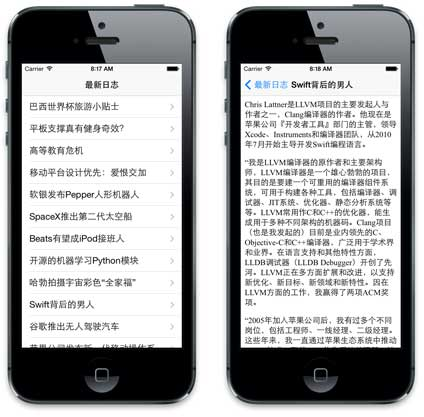
\includegraphics[width=0.6\linewidth]{fig/956198702546240.png}
\end{figure}


只需要调用 API:\texttt{/api/blogs}。

在 XCode 中完成 App 编写:

 
 \begin{figure}[htp]
	\centering
	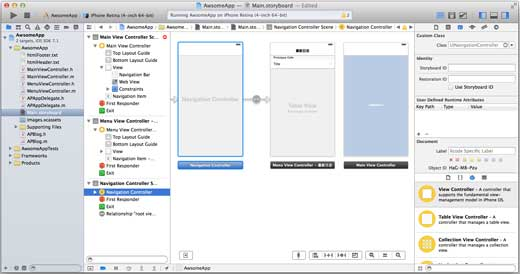
\includegraphics[width=0.6\linewidth]{fig/956198878703904.png}
\end{figure}


由于我们的教程是 Python,关于如何开发 iOS,请移步
\href{https://developer.apple.com/technologies/ios/}{Develop Apps for
iOS}。

\href{https://github.com/michaelliao/awesome-python3-webapp/tree/day-16/ios}{点击下载
iOS App 源码}。

如何编写 Android App?这个当成作业了。

\hypertarget{ux53c2ux8003ux6e90ux7801}{%
\subsubsection{参考源码}\label{ux53c2ux8003ux6e90ux7801}}

\href{https://github.com/michaelliao/awesome-python3-webapp/tree/day-16}{day-16}

